\colorlet{circle edge}{black!50}
\colorlet{circle area}{gray!20}

\tikzset{
  filled/.style={fill=circle area, 
  %draw=circle edge, 
  thick},
  outline/.style={draw=circle edge, thick}
  }

\setlength{\parskip}{5mm}

\tikzstyle{edge} = [draw, thick, -]
\tikzstyle{vertex}=[circle,fill=black!50,minimum size=10pt,inner sep=0pt]
\tikzstyle{selected edge} = [draw, line width=2cm,-,gray!20] 


\subfloat[Linear Swept Sphere]{\label{fig:rdr1}
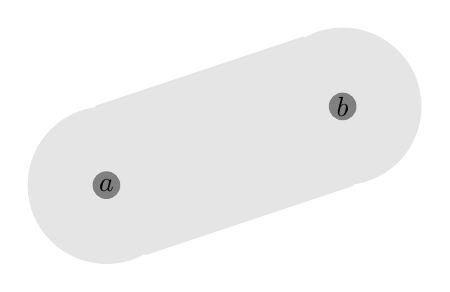
\begin{tikzpicture}  

    % Definition of the radii
    \def\firstradius{(0,0) circle (1cm)};
    \def\secondradius{(3, 1) circle (1cm)};

    \fill[filled] \firstradius;
    \fill[filled] \secondradius;
 
    \foreach \pos/\name in {{(0,0)/a}, {(3, 1)/b}} {   
      \node[vertex] (\name) at \pos {$\name$};
    }
   
    \path[selected edge] (a) -- (b);
\end{tikzpicture}}
% Remove empty line
\subfloat[Circle]{\label{fig:rdr2}
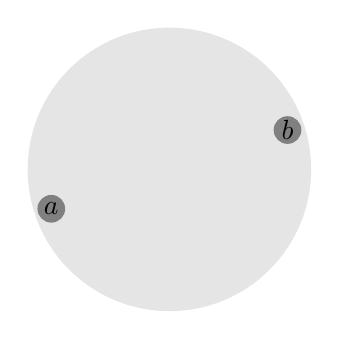
\begin{tikzpicture}  

    % Definition of the radii
    \def\radius{(1.5,0.5) circle (1.8)};
    \fill[filled] \radius;
 
    \foreach \pos/\name in {{(0,0)/a}, {(3, 1)/b}} {   
      \node[vertex] (\name) at \pos {$\name$};
    }   
\end{tikzpicture}}
% Remove empty line
\subfloat[Rectangle]{\label{fig:rdr3}
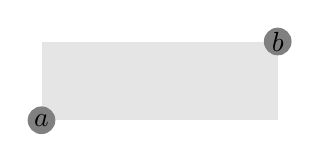
\begin{tikzpicture}  

    % Definition of the radii
    \def\rectangle{(0,0) rectangle (3,1)};
    \fill[filled] \rectangle;
 
    \foreach \pos/\name in {{(0,0)/a}, {(3, 1)/b}} {   
      \node[vertex] (\name) at \pos {$\name$};
    }   
\end{tikzpicture}}
